% !TeX program = xelatex
% 编译：xelatex 02-典型的系统.tex（VS Code 的 LaTeX Workshop 会读上一行，自动用 xelatex）
% 来源：2022 浙江大学《信号与系统》胡浩基老师，教材第 28 页「系统的基本性质」一节课及后两堂课，视频 00:00--121:33（线性、时不变、因果、无记忆、可逆、稳定，加最后的习题复习）。
% 体例：每个性质按「概念 → 证明（方法/判据）→ 例题」组织。
\documentclass[UTF8,a4paper,11pt]{ctexart}
\usepackage{amsmath,amssymb}
\usepackage{geometry}
\geometry{margin=2.4cm}
\usepackage{xcolor}
\usepackage{mdframed}
\usepackage{booktabs}
\usepackage{enumitem}
\usepackage{tikz}
\usetikzlibrary{arrows.meta,positioning,calc}
\usepackage{float}
\usepackage{fancyhdr}
% 页眉页脚清空，只在右下角保留页号（含首页）
\fancypagestyle{plain}{%
  \fancyhf{}%
  \fancyfoot[R]{\thepage}%
  \renewcommand{\headrulewidth}{0pt}%
  \renewcommand{\footrulewidth}{0pt}}
\usepackage{needspace}% 例题标题后紧跟表格时，避免标题被留在页底
\usepackage[hidelinks,unicode,bookmarksnumbered,bookmarksopen=true,bookmarksopenlevel=2,pdftitle={典型的系统：线性、时不变、因果、无记忆、可逆、稳定}]{hyperref}
\usepackage{bookmark}% XeTeX 下 hyperref 自带的大纲不生效，用 bookmark 宏包生成 PDF 书签（需编译两遍）

\setCJKmainfont{Songti SC}[BoldFont={Songti SC Bold}]
\setCJKsansfont{PingFang SC}

\newmdenv[backgroundcolor=blue!4,linecolor=blue!50!black,linewidth=1pt,innertopmargin=6pt,innerbottommargin=6pt]{rememberbox}
\newenvironment{remember}{\begin{rememberbox}\textbf{重点}\par\smallskip}{\end{rememberbox}}
\newmdenv[backgroundcolor=yellow!8,linecolor=orange!70!black,linewidth=1pt,innertopmargin=6pt,innerbottommargin=6pt]{notebox}
\newenvironment{note}{\begin{notebox}\textbf{说明}\par\smallskip}{\end{notebox}}
\newmdenv[backgroundcolor=gray!8,linecolor=gray!60,linewidth=0.8pt,innertopmargin=5pt,innerbottommargin=5pt]{skipbox}
\newenvironment{skippable}{\begin{skipbox}\textbf{可跳过}\par\smallskip}{\end{skipbox}}

% ---------------------------------------------------------------- 标题层级
% 章(section)、小节(subsection)：深蓝；例题：橙色徽章；小标题：青色三角。三者颜色和形状都不同，一眼能分清。
\definecolor{secblue}{RGB}{31,78,121}
\definecolor{exorange}{RGB}{190,90,10}
\definecolor{ptteal}{RGB}{0,110,110}
\ctexset{
  section={format=\raggedright\Large\bfseries\color{secblue},
           beforeskip=3.2ex plus 1ex minus .5ex, afterskip=1.4ex,
           aftertitle={\par\nobreak\vspace{-1.1ex}\noindent\textcolor{secblue}{\rule{\linewidth}{0.8pt}}\par\nobreak\vspace{0.6ex}}},
  subsection={format=\raggedright\large\bfseries\color{secblue},
              beforeskip=2.4ex plus .8ex minus .4ex, afterskip=1.0ex}
}
% 例题标题：\example{标题}{结论}{视频时刻}。左边橙色实心「例 n」，右边结论标签；同时进 PDF 大纲（第 3 级）。
\newcounter{ex}[section]
\newcommand{\example}[3]{%
  \refstepcounter{ex}\phantomsection
  \addcontentsline{toc}{subsubsection}{例 \theex\ #1（#2）}%
  \par\addvspace{1.6ex}\noindent
  {\setlength{\fboxsep}{3pt}%
   \colorbox{exorange}{\textcolor{white}{\textbf{例~\theex}}}\ %
   \textcolor{exorange}{\textbf{#1}}\ {\footnotesize\textcolor{gray!70!black}{#3}}%
   \hfill\colorbox{exorange!12}{\small\textcolor{exorange}{#2}}\par}%
  \nobreak\vskip0.6ex\relax\csname @afterheading\endcsname}
% 小标题（不是章节也不是例题）：青色三角 + 粗体，接着同一段往下写，不进大纲。
\newcommand{\point}[1]{\par\addvspace{1ex}\noindent\textcolor{ptteal}{$\blacktriangleright$\,\textbf{#1}}\ }

% ---------------------------------------------------------------- 画图用的小宏
% 一行「输入 -> 系统 -> 输出」。#1 纵坐标，#2 输入，#3 输出，#4 右侧备注（灰字）
\newcommand{\sysline}[4]{%
  \node[anchor=east] at (2.9,#1) {#2};
  \draw[->,thick] (3.0,#1) -- (3.8,#1);
  \node[draw,rounded corners=2pt,fill=blue!6,minimum width=1.3cm,minimum height=0.62cm] at (4.45,#1) {\small 系统};
  \draw[->,thick] (5.1,#1) -- (5.9,#1);
  \node[anchor=west] at (6.0,#1) {#3};
  \node[anchor=west,gray!55!black,font=\footnotesize] at (9.4,#1) {#4};}

\title{典型的系统：线性、时不变、因果、无记忆、可逆、稳定\\\large 浙江大学 2022《信号与系统》（胡浩基）教材第 28 页「系统的基本性质」听课笔记}
\author{}
\date{}

\begin{document}
\pagestyle{plain}
\maketitle

%==================================================================
\section{概览：6 对性质}
一个\textbf{系统}(system)是一台机器：信号 $x(t)$ 进去，信号 $y(t)$ 出来。后面所有性质，都是在问「这台机器有什么脾气」。6 对性质每一对都\textbf{非此即彼}（不是线性就是非线性，以此类推），所以只要把正面的定义写严格就够了。

\begin{center}
\begin{tabular}{@{}ll@{}}
\toprule
性质 & 反面\\
\midrule
线性系统(linear system) & 非线性系统(nonlinear system)\\
时不变系统(time-invariant system) & 时变系统(time-varying system)\\
因果系统(causal system) & 非因果系统(non-causal system)\\
无记忆系统(memoryless system) & 记忆系统(system with memory)\\
可逆系统(invertible system) & 不可逆系统\\
稳定系统(stable system) & 不稳定系统\\
\bottomrule
\end{tabular}
\end{center}

%==================================================================
\section{线性系统}
\subsection{概念}
\begin{remember}
一个系统，如果\textbf{同时}满足下面两条，它就是线性系统；否则（只满足一条，或两条都不满足）就是非线性系统。

\medskip
假设对\textbf{任意}输入 $x(t)$，系统给出输出 $y(t)$（记作 $x(t)\to y(t)$），那么：
\begin{enumerate}[nosep]
\item \textbf{齐次性}(homogeneity)：$a\,x(t)\to a\,y(t)$，其中 $a$ 是任意实数。\\
\hfill\emph{输入放大 $a$ 倍，输出也恰好放大 $a$ 倍。}
\item \textbf{叠加性}(superposition，也叫可加性)：若 $x_1(t)\to y_1(t)$、$x_2(t)\to y_2(t)$，则 $x_1(t)+x_2(t)\to y_1(t)+y_2(t)$。\\
\hfill\emph{两个输入加在一起送进去，输出就是它们各自输出的和。}
\end{enumerate}
\end{remember}

\begin{figure}[H]
\centering
\begin{tikzpicture}[>=stealth]
  \sysline{0}{$x(t)$}{$y(t)$}{这是出发点}
  \sysline{-1.0}{$a\,x(t)$}{$a\,y(t)$}{齐次性：输入乘 $a$，输出也乘 $a$}
  \draw[gray!50,dashed] (0.3,-1.65) -- (15.3,-1.65);
  \sysline{-2.3}{$x_1(t)$}{$y_1(t)$}{各自送进去，各自得到}
  \sysline{-3.1}{$x_2(t)$}{$y_2(t)$}{}
  \sysline{-4.1}{$x_1(t)+x_2(t)$}{$y_1(t)+y_2(t)$}{叠加性：和送进去，得到和}
\end{tikzpicture}
\caption{线性系统的两条规矩。注意每一行里的「系统」都是\textbf{同一台}机器。}
\end{figure}

两点要记住：
\begin{itemize}[nosep]
\item \textbf{缺一不可}：只有齐次性和叠加性同时满足才是线性（见本节末的思考题）。
\item \textbf{「任意」是定义的灵魂}：$x(t)$、$x_1(t)$、$x_2(t)$、$a$ 都是任意的（记作 $\forall$）。后面所有难点，都出在没有真正理解这个「任意」。例如 $y(t)=3x(t)$ 的意思是：这台机器对\textbf{任意}输入都乘 3。
\end{itemize}
离散线性系统的定义只需把圆括号 $(t)$ 换成方括号 $[n]$：$x[n]\to y[n]$，$a\,x[n]\to a\,y[n]$，$x_1[n]+x_2[n]\to y_1[n]+y_2[n]$。

\subsection{证明}
\begin{remember}
\textbf{证}一个系统是线性的：对\textbf{所有}输入、\textbf{所有} $a$ 都验证两条规矩，一条也不能漏。

\textbf{证}一个系统不是线性的：只要找到\textbf{一个}反例，让它不满足齐次性或叠加性之一，就够了。

原因就是定义里的「任意」：说「对任意都成立」要全部验完；说「不是对任意都成立」，有一个例外就够。
\end{remember}

\point{证线性：设中间变量，打成「一包」。}
先看清这台机器的规矩：「送进去信号 $f$，出来 $F[f]$」（例如放大器：送进去 $f$，出来 $3f$）。因为 $x(t)$ 是任意信号，所以 $a\,x(t)$ 也\textbf{只是又一个信号}；设中间变量 $f(t)=a\,x(t)$，把它当成一包整体送进去，再做代换。步骤：
\begin{enumerate}[nosep]
\item 齐次性：令 $f=a\,x(t)$，算出 $F[f]$，化成 $a\,y(t)$；
\item 叠加性：令 $f=x_1(t)+x_2(t)$，算出 $F[f]$，化成 $y_1(t)+y_2(t)$。
\end{enumerate}

\point{证非线性：对照「实际」和「希望」。}
取最简单的输入（如 $x\equiv0$ 或 $x\equiv1$，$\equiv$ 表示恒等于）和 $a=2$：\textbf{实际}是把 $a\,x$ 送进系统得到的输出；\textbf{希望}是「若齐次性成立，应得 $a\,y$」。两者不等，就矛盾，说明系统不是线性的。

\subsection{例题：证明是线性}
下面每题都按定义分\textbf{齐次性}、\textbf{叠加性}两步，写成证明。

\example{放大器~\texorpdfstring{$y(t)=3x(t)$}{y(t)=3x(t)}}{线性}{}
\textbf{系统}：$x(t)\to y(t)=3x(t)$，即输入乘 $3$。

\textbf{证明}。
\begin{align*}
\text{齐次性：}\quad & a\,x(t)\ \to\ 3\cdot a\,x(t)=a\cdot 3x(t)=a\,y(t),\\
\text{叠加性：}\quad & x_1(t)+x_2(t)\ \to\ 3\bigl(x_1(t)+x_2(t)\bigr)=3x_1(t)+3x_2(t)=y_1(t)+y_2(t).
\end{align*}
两式对任意输入、任意实数 $a$ 均成立，故 $y(t)=3x(t)$ 为线性系统。\hfill$\blacksquare$

\example{\texorpdfstring{$y(t)=t\,x(t)$}{y(t)=t x(t)}}{线性}{}
\textbf{系统}：$x(t)\to y(t)=t\,x(t)$。$t$ 是每个时刻的乘数，不随输入改变。

\textbf{证明}。
\begin{align*}
\text{齐次性：}\quad & a\,x(t)\ \to\ t\cdot a\,x(t)=a\bigl(t\,x(t)\bigr)=a\,y(t),\\
\text{叠加性：}\quad & x_1(t)+x_2(t)\ \to\ t\bigl(x_1(t)+x_2(t)\bigr)=t\,x_1(t)+t\,x_2(t)=y_1(t)+y_2(t).
\end{align*}
两式对任意输入、任意实数 $a$ 均成立，故 $y(t)=t\,x(t)$ 为线性系统。\hfill$\blacksquare$

\textbf{注}：$t$ 随时间变化不影响线性——线性只问「放大或相加时，输出是否跟着放大或相加」，$t$ 只是逐点的系数；它的影响体现在时不变性上（见下一节的 $y(t)=t\,x(t)$）。

\example{微分器~\texorpdfstring{$y(t)=\dfrac{\mathrm{d}x(t)}{\mathrm{d}t}$}{y(t)=dx(t)/dt}}{线性}{}
\textbf{系统}：$x(t)\to y(t)=\dfrac{\mathrm{d}x(t)}{\mathrm{d}t}$。

\textbf{证明}。用微分的线性：
\begin{align*}
\text{齐次性：}\quad & \frac{\mathrm{d}}{\mathrm{d}t}\bigl[a\,x(t)\bigr]=a\frac{\mathrm{d}x(t)}{\mathrm{d}t}=a\,y(t),\\
\text{叠加性：}\quad & \frac{\mathrm{d}}{\mathrm{d}t}\bigl[x_1(t)+x_2(t)\bigr]=\frac{\mathrm{d}x_1(t)}{\mathrm{d}t}+\frac{\mathrm{d}x_2(t)}{\mathrm{d}t}=y_1(t)+y_2(t).
\end{align*}
故微分器为线性系统。\hfill$\blacksquare$

\example{积分器~\texorpdfstring{$y(t)=\displaystyle\int_{-\infty}^{t}x(\tau)\,\mathrm{d}\tau$}{y(t)=∫x(τ)dτ}}{线性}{}
\textbf{系统}：$x(t)\to y(t)=\displaystyle\int_{-\infty}^{t}x(\tau)\,\mathrm{d}\tau$。

\textbf{证明}。用积分的线性（常数可提出，和的积分等于积分的和）：
\begin{align*}
\text{齐次性：}\quad & \int_{-\infty}^{t}a\,x(\tau)\,\mathrm{d}\tau=a\int_{-\infty}^{t}x(\tau)\,\mathrm{d}\tau=a\,y(t),\\
\text{叠加性：}\quad & \int_{-\infty}^{t}\bigl[x_1(\tau)+x_2(\tau)\bigr]\mathrm{d}\tau=\int_{-\infty}^{t}x_1(\tau)\,\mathrm{d}\tau+\int_{-\infty}^{t}x_2(\tau)\,\mathrm{d}\tau=y_1(t)+y_2(t).
\end{align*}
故积分器为线性系统。\hfill$\blacksquare$

\needspace{6cm}
\example{离散的四个系统}{线性}{}
把前面几个系统改写成离散形式：
\begin{center}
\begin{tabular}{@{}lll@{}}
\toprule
系统 & 在做什么 & 结论\\
\midrule
$y[n]=2x[n]$ & 每个数乘 2 & 线性，证法同 $3x(t)$\\
$y[n]=n\,x[n]$ & 第 $n$ 个数乘 $n$ & 线性，证法同 $t\,x(t)$\\
$y[n]=x[n]-x[n-1]$ & 当前值减前一个值（\textbf{差分}） & 线性，下面完整证\\
$y[n]=\displaystyle\sum_{k=-\infty}^{n}x[k]$ & 从最早加到现在（\textbf{累加}） & 线性，留作练习\\
\bottomrule
\end{tabular}
\end{center}
差分(difference)就是离散的微分器（离散信号没法求导，「后一个减前一个」就是近似的求导）；累加(accumulator)就是离散的积分器。

\point{差分 $y[n]=x[n]-x[n-1]$ 的证明。}
\begin{itemize}[nosep]
\item 齐次性：输入 $a\,x[n]$，输出 $a\,x[n]-a\,x[n-1]=a\bigl(x[n]-x[n-1]\bigr)=a\,y[n]$；
\item 叠加性：输入 $x_1[n]+x_2[n]$，输出 $\bigl(x_1[n]-x_1[n-1]\bigr)+\bigl(x_2[n]-x_2[n-1]\bigr)=y_1[n]+y_2[n]$。
\end{itemize}
故差分为线性系统。\hfill$\blacksquare$

\subsection{例题：证明不是线性}
\example{\texorpdfstring{$y(t)=x(t)+1$}{y(t)=x(t)+1}}{非线性}{}
\textbf{系统}：$x(t)\to y(t)=x(t)+1$。

\textbf{证明}（举反例）。取 $x(t)\equiv0$、$a=2$：
\begin{itemize}[nosep]
\item 输入 $x(t)\equiv0$，输出 $y(t)=0+1=1$；
\item 输入 $2x(t)\equiv0$，与原输入是\textbf{同一个信号}，实际输出仍为 $1$；
\item 若齐次性成立，应有 $a\,y(t)=2\times1=2$。
\end{itemize}
实际输出 $1\neq$ 期望值 $2$，故齐次性不成立，$y(t)=x(t)+1$ 为非线性系统。\hfill$\blacksquare$

\begin{figure}[H]
\centering
\begin{tikzpicture}[>=stealth]
  \sysline{0}{$x(t)\equiv0$}{$1$}{实际：$0+1=1$}
  \sysline{-1.0}{$2x(t)\equiv0$}{$\mathbf{1}$（实际）}{实际：$0+1=1$}
  \node[anchor=west,red!70!black,font=\footnotesize] at (6.0,-1.55) {若齐次性成立，应得 $2\times1=\mathbf{2}$（希望）};
  \node[anchor=west,red!70!black,font=\footnotesize] at (6.0,-2.0) {实际 $1\neq$ 希望 $2$，所以不是线性系统};
\end{tikzpicture}
\caption{反例 $y(t)=x(t)+1$：输入是同一个全零信号，输出却被要求同时等于 $1$ 和 $2$。}
\end{figure}

\example{\texorpdfstring{$y(t)=x(t)^2$}{y(t)=x(t)的平方}}{非线性}{}
\textbf{系统}：$x(t)\to y(t)=x(t)^2$。

\textbf{证明}（举反例）。取 $x(t)\equiv1$、$a=2$：
\begin{align*}
\text{实际：}\quad & x(t)\equiv1\ \to\ y(t)=1^2=1,\qquad 2x(t)\equiv2\ \to\ 2^2=4;\\
\text{期望：}\quad & a\,y(t)=2\times1=2.
\end{align*}
实际输出 $4\neq$ 期望值 $2$，故齐次性不成立，$y(t)=x(t)^2$ 为非线性系统。\hfill$\blacksquare$

\begin{figure}[H]
\centering
\begin{tikzpicture}[>=stealth]
  \sysline{0}{$x(t)\equiv1$}{$1^2=1$}{实际}
  \sysline{-1.0}{$2x(t)\equiv2$}{$2^2=\mathbf{4}$（实际）}{实际}
  \node[anchor=west,red!70!black,font=\footnotesize] at (6.0,-1.55) {若齐次性成立，应得 $2\times1=\mathbf{2}$（希望）};
  \node[anchor=west,red!70!black,font=\footnotesize] at (6.0,-2.0) {实际 $4\neq$ 希望 $2$，所以不是线性系统};
\end{tikzpicture}
\caption{反例 $y(t)=x(t)^2$：输入翻一倍，输出翻了\textbf{四}倍。}
\end{figure}

\begin{skippable}
\textbf{快速检查：全零输入必须得到全零输出}。齐次性里 $a$ 可取 $0$，所以线性系统对零输入一定给零输出；$y(t)=x(t)+1$ 就栽在这里。反过来\textbf{不成立}：$y(t)=x(t)^2$ 对零输入给零，却不是线性的。所以这个检查只能「判死刑」，不能「判线性」。
\end{skippable}

\subsection{应付考试的判据：两句话}
这个办法不能覆盖所有系统，但能覆盖 70\%--80\% 以上。

\begin{remember}
线性系统的判据：
\begin{enumerate}[nosep]
\item \textbf{每一项都有 $x$}；
\item \textbf{每一项的 $x$ 都是一次}。
\end{enumerate}
\end{remember}

\begin{figure}[H]
\centering
\begin{tikzpicture}[>=stealth,
  box/.style={draw,rounded corners=3pt,align=center,minimum height=0.9cm,inner sep=5pt},
  yes/.style={font=\footnotesize,green!40!black},
  no/.style={font=\footnotesize,red!70!black}]
  \node[box,fill=gray!8] (a) at (0,0) {拿到一个系统\\ $y=\cdots$};
  \node[box,fill=blue!6] (b) at (3.9,0) {\textbf{第 1 句}：每一项\\都有 $x$ 吗？};
  \node[box,fill=blue!6] (c) at (9.3,0) {\textbf{第 2 句}：每一项的 $x$\\都是一次吗？};
  \node[box,fill=green!10] (d) at (13.6,-2.0) {线性};
  \node[box,fill=red!10] (e) at (3.9,-2.0) {非线性};
  \node[box,fill=red!10] (f) at (9.3,-2.0) {非线性};
  \draw[->] (a) -- (b);
  \draw[->] (b) -- node[above,yes] {都有} (c);
  \draw[->] (b) -- node[right,no] {有一项没有} (e);
  \draw[->] (c) -- node[right,no] {有一项不是一次} (f);
  \draw[->] (c) -| node[above,pos=0.2,yes] {都是一次} (d);
\end{tikzpicture}
\caption{线性系统的两句话判断法。}
\end{figure}

\begin{center}
\begin{tabular}{@{}lll@{}}
\toprule
系统 & 两句话检查 & 结论\\
\midrule
$y(t)=3x(t)+2x(t-2)$ & 两项都有 $x$，都是一次 & 线性\\
$y[n]=n\,x[n-2]+3x[n+1]$ & 两项都有 $x$，都是一次（$n$ 是系数，不是 $x$） & 线性\\
$y(t)=3x(t)+2$ & 第二项「$2$」\textbf{没有 $x$} & 非线性\\
$y[n]=e^{x[n]}$ & 看起来「有 $x$，也只出现一次」，\textbf{但要展开看} & 非线性\\
\bottomrule
\end{tabular}
\end{center}

\point{为什么 $e^{x[n]}$ 看起来像线性却不是。}
$e^{x}=1+x+\dfrac{x^2}{2!}+\cdots$（泰勒展开，Taylor expansion），里面有常数项 $1$（没有 $x$）、有 $x^2$（不是一次），两句话都不满足，所以非线性。两句话要看\textbf{展开以后}每一项的样子，不是看表面写法。

\begin{skippable}
\textbf{两句话的边界}：$x$ 被套在函数里，如 $|x(t)|$、$\sin x(t)$，和 $e^{x}$ 是同一类陷阱；两个 $x$ 相乘，如 $x(t)\,x(t-1)$，「一次」就不满足；真要严格证明，还是回到齐次 + 叠加。
\end{skippable}

\subsection{与教材定义的等价}
教材把两条合成一条（教材第 28 页，式 1-89、1-90）。两种定义\textbf{完全等价}，关键在「任意」。

\begin{center}
\renewcommand{\arraystretch}{1.3}
\begin{tabular}{@{}p{2.2cm}p{12.6cm}@{}}
\toprule
 & 内容\\
\midrule
分开写 & 两条分开写：齐次性 $x(t)\to y(t)\Rightarrow a\,x(t)\to a\,y(t)$；叠加性 $x_1\to y_1,\ x_2\to y_2\Rightarrow x_1+x_2\to y_1+y_2$。\\
合并写 & 一条合起来写：对任意 $x_1\to y_1$、$x_2\to y_2$ 和任意实数 $a,b$，都有 $a\,x_1(t)+b\,x_2(t)\to a\,y_1(t)+b\,y_2(t)$。\\
\bottomrule
\end{tabular}
\end{center}

\begin{figure}[H]
\centering
\begin{tikzpicture}[>=stealth,
  box/.style={draw,rounded corners=4pt,align=center,minimum width=5.4cm,minimum height=1.6cm,inner sep=6pt}]
  \node[box,fill=blue!6] (L) at (0,0) {\textbf{书上定义}\\ $a\,x_1+b\,x_2\to a\,y_1+b\,y_2$\\ 对任意 $a,b$};
  \node[box,fill=green!8] (R) at (9.2,0) {\textbf{分开写}\\ 齐次性 + 叠加性};
  \draw[->,thick,bend left=22] (L.north east) to node[above,align=center,font=\footnotesize] {特殊情况：取 $a=1,b=0$ 得齐次性\\ 取 $a=b=1$ 得叠加性} (R.north west);
  \draw[->,thick,bend left=22] (R.south west) to node[below,align=center,font=\footnotesize] {先对 $x_1$ 用齐次，对 $x_2$ 用齐次\\ 再把两个「包」用叠加加起来} (L.south east);
\end{tikzpicture}
\caption{两个定义互相推得出对方，所以说它们等价。}
\end{figure}

\point{合并写 $\Rightarrow$ 分开写（简单）。}
取 $b=0$（$a$ 任意），$x_1=x$：$a\,x+0\to a\,y+0$，即齐次性 $a\,x\to a\,y$。取 $a=b=1$：直接得到叠加性。

\point{分开写 $\Rightarrow$ 合并写（稍难）。}
\textbf{已知}（分开写的定义，对\textbf{任意}输入都成立）。为避免和后面的 $a,b$ 混淆，齐次性里的倍数换用字母 $c$：
\begin{itemize}[nosep]
\item[(H)] 齐次性：若 $x\to y$，则对任意实数 $c$，有 $c\,x\to c\,y$；
\item[(S)] 叠加性：若 $x_A\to y_A$、$x_B\to y_B$，则 $x_A+x_B\to y_A+y_B$。
\end{itemize}
\textbf{要证}（书上的定义）：任取 $x_1\to y_1$、$x_2\to y_2$，任取实数 $a,b$，都有
\[
a\,x_1(t)+b\,x_2(t)\ \to\ a\,y_1(t)+b\,y_2(t).
\]
\textbf{证明}。分三步，只用 (H) 和 (S)，完全不去管系统「里面」具体是什么运算：
\begin{enumerate}
\item \textbf{对 $x_1$ 用 (H)，取 $c=a$。}$x_1$ 是任意输入，已知 $x_1\to y_1$，所以 (H) 对它成立：
\[
a\,x_1(t)\ \to\ a\,y_1(t).
\]
\item \textbf{对 $x_2$ 用 (H)，取 $c=b$。}$x_2$ 也是任意输入，已知 $x_2\to y_2$，$b$ 是任意实数，所以
\[
b\,x_2(t)\ \to\ b\,y_2(t).
\]
\item \textbf{把前两步的结果当作两个输入，用 (S)。}令 $u(t)=a\,x_1(t)$，$v(t)=b\,x_2(t)$。它们各自只是一个信号（「一包」）；由第 1、2 步，$u\to a\,y_1$，$v\to b\,y_2$。(S) 对\textbf{任意}两个输入都成立，取 $x_A=u$、$x_B=v$，$y_A=a\,y_1$、$y_B=b\,y_2$，得
\[
u+v\ \to\ a\,y_1+b\,y_2,\qquad\text{即}\qquad a\,x_1(t)+b\,x_2(t)\ \to\ a\,y_1(t)+b\,y_2(t).
\]
\end{enumerate}
$x_1,x_2,a,b$ 都是任取的，所以书上的定义对\textbf{任意}输入、任意 $a,b$ 成立。证毕。

\begin{figure}[H]
\centering
\begin{tikzpicture}[>=stealth]
  \sysline{0}{$x_1$}{$y_1$}{已知}
  \sysline{-0.9}{$x_2$}{$y_2$}{已知}
  \draw[gray!50,dashed] (0.3,-1.45) -- (13.3,-1.45);
  \sysline{-2.0}{$a\,x_1$}{$a\,y_1$}{第 1 步：(H)，取 $c=a$}
  \sysline{-2.9}{$b\,x_2$}{$b\,y_2$}{第 2 步：(H)，取 $c=b$}
  \draw[gray!50,dashed] (0.3,-3.45) -- (13.3,-3.45);
  \sysline{-4.0}{$a\,x_1+b\,x_2$}{$a\,y_1+b\,y_2$}{第 3 步：(S)，把 $a\,x_1$、$b\,x_2$ 当两个输入}
\end{tikzpicture}
\caption{分开写 $\Rightarrow$ 合并写：先用齐次性分别把 $x_1$、$x_2$ 放大成 $a\,x_1$、$b\,x_2$，再用叠加性把两个放大后的信号加起来。每一行的「系统」仍是\textbf{同一台}机器。}
\end{figure}

\point{几个容易卡住的地方}
\begin{itemize}[nosep]
\item \textbf{为什么能对 $x_1$ 用 (H)}：(H) 里的 $x$ 是\textbf{任意}输入，$x_1$ 就是其中一个；(H) 里的 $c$ 是任意实数，取成 $a$ 当然允许（$a=0$ 或负数也行）。这就是「任意」的用法：把定义里的字母换成手头的具体信号和数。
\item \textbf{第 1 步的输出 $a\,y_1$ 是 (H) 保证的}，不是我们自己去算 $a\,x_1$ 经过系统得到的；我们根本不知道系统内部怎么算，只知道 (H)。
\item \textbf{第 3 步为什么不是「直接相加」}：$a\,x_1$ 和 $b\,x_2$ 的输出 $a\,y_1$、$b\,y_2$ 是第 1、2 步得到的结论；要把「两个输入的和」对应到「两个输出的和」，靠的是 (S)，不能省。(S) 只管「两个输入相加」，所以要先用 (H) 把 $a,b$ 吸收进信号里，凑成 (S) 的形状。
\end{itemize}
若觉得绕、烧脑，核心是没有理解「任意」。日常用哪个都行：分开写更适合入门证明，合并写更适合推别的结论。

\subsection{课后思考题：缺一不可}
\begin{remember}
\begin{enumerate}[nosep]
\item 请举一个系统，\textbf{满足齐次性，不满足叠加性}；
\item 请再举一个系统，\textbf{满足叠加性，不满足齐次性}。
\end{enumerate}
\end{remember}
这是第一次作业里的一道思考题，两道里\textbf{有一道特别难}（提示：$a$ 可取负数）。

\begin{skippable}
\textbf{第 1 道}：$y(t)=\dfrac{x(t)^2}{x(t-1)}$（分母为 $0$ 时约定输出 $0$）满足齐次性：$\dfrac{a^2x(t)^2}{a\,x(t-1)}=a\cdot\dfrac{x(t)^2}{x(t-1)}$；但取某一时刻 $(x_1(t),x_1(t-1))=(1,1)$、$(x_2(t),x_2(t-1))=(1,2)$，则 $y_1=1$、$y_2=\tfrac12$，而和的输出是 $\tfrac{2^2}{3}=\tfrac43\neq\tfrac32$，叠加性不成立。第 2 道很难：$a$ 取任意实数时，叠加性已能推出整数、分数的齐次性，反例只能靠「病态」函数（柯西函数方程的非线性解，需借助选择公理）。
\end{skippable}

%==================================================================
\section{时不变系统}
\subsection{概念}
\begin{remember}
假设对\textbf{任意}输入 $x(t)$，系统给出输出 $y(t)$。如果对\textbf{任意实数} $t_0$，都有
\[
x(t-t_0)\ \to\ y(t-t_0),
\]
那么它是\textbf{时不变系统}(time-invariant system)；否则是\textbf{时变系统}(time-varying system)。

\emph{大白话：输入晚到 $t_0$ 秒，输出也恰好晚 $t_0$ 秒，形状一点不变。}
\end{remember}
$x(t-t_0)$ 就是把 $x$ \textbf{右移 $t_0$ 个单位}（$t_0$ 为负则左移）。

时不变：同样的输入无论何时送入，输出都一样；若输出随送入时刻改变，就是时变。系统的输出不随输入送入的时刻而改变。

\begin{figure}[H]
\centering
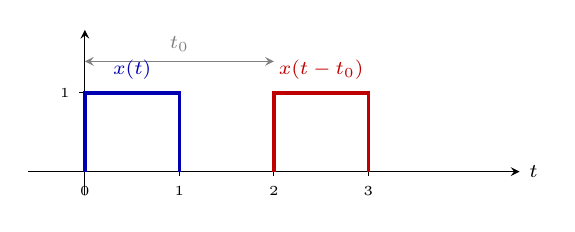
\begin{tikzpicture}[x=1.2cm,y=1.0cm,>=stealth]
  \draw[->] (-0.6,0) -- (4.6,0) node[right,font=\scriptsize] {$t$};
  \draw[->] (0,-0.3) -- (0,1.8);
  \foreach \k in {0,1,2,3} { \draw (\k,0.06) -- (\k,-0.06) node[below,font=\tiny] {$\k$}; }
  \draw (0.06,1) -- (-0.06,1) node[left,font=\tiny] {$1$};
  \draw[very thick,blue!70!black] (0,0) -- (0,1) -- (1,1) -- (1,0);
  \draw[very thick,red!75!black] (2,0) -- (2,1) -- (3,1) -- (3,0);
  \draw[<->,gray] (0,1.4) -- (2,1.4) node[midway,above,font=\scriptsize] {$t_0$};
  \node[font=\scriptsize,blue!70!black,anchor=south] at (0.5,1.05) {$x(t)$};
  \node[font=\scriptsize,red!75!black,anchor=south] at (2.5,1.05) {$x(t-t_0)$};
\end{tikzpicture}
\caption{时不变：输入整体右移 $t_0$，输出也只是同样右移 $t_0$，形状不变，即 $x(t-t_0)\to y(t-t_0)$。}
\end{figure}

\subsection{证明}
\begin{remember}
\textbf{证}时不变：必须严格按定义证。设中间变量 $f(t)=x(t-t_0)$，代进系统的规矩，得到「实际」输出；再把 $y(t)$ 里所有的 $t$ 换成 $t-t_0$，得到「希望」输出。两边相等就是时不变。

\textbf{证}时变：举一个反例，列出「实际」和「希望」，二者不等即可。
\end{remember}

\subsection{做题步骤：固定写两行}
\textbf{固定写两行，按部就班不容易代错。}
\begin{enumerate}[nosep]
\item \textbf{先用口诀预判}：$x$ 括号外有没有随 $t$ 变的项？括号里是不是只有 $t$ 加减常数？两条都过，多半时不变；有一条不过，多半时变。带积分或求和的系统口诀不灵，直接走下面几步（积分要换元，例子见例~\ref{ex:int}）。
\item \textbf{写出系统规矩}：用中间变量 $f$ 表示「送进来的任意信号」，把系统写成 $f(t)\to\cdots$。例：$x(2t)$ 写成 $f(t)\to f(2t)$；$t\,x(t)$ 写成 $f(t)\to t\,f(t)$。
\item \textbf{第一行，写「实际」}（先移输入，再过系统）：令 $f(t)=x(t-t_0)$，先写出它的入口规则 $f(\square)=x(\square-t_0)$，再把系统规矩里要的东西填进 $\square$。系统自带的东西（$2t$ 里的 $2$、$\cos t$、单独的 $t$）\textbf{原样保留，不跟着 $t_0$ 动}。
\item \textbf{第二行，写「期望」}（先过系统，再移输出）：先写出 $y(\square)$ 的规则，再把 $\square$ 换成 $t-t_0$：$y(t)$ 里\textbf{所有}的 $t$ 一起换。
\item \textbf{比较两行}。对任意 $t_0$ 都相等，是时不变，$\blacksquare$；不等，是时变。证时变时再取一个具体的 $x$（矩形脉冲、阶跃、单位脉冲）和一个具体的 $t_0$（如 $1$），算出两个不同的结果，$\blacksquare$。
\end{enumerate}

\textbf{时变的两种来源}（看到哪一种，就知道「实际」和「期望」会在哪里分家）：
\begin{center}
\renewcommand{\arraystretch}{1.3}
\begin{tabular}{@{}p{3.6cm}p{3.6cm}p{7.2cm}@{}}
\toprule
类型 & 例子 & 为什么「实际」$\neq$「期望」\\
\midrule
对 $t$ 缩放或反转 & $x(2t)$、$x(-t)$、$x[3-n]$ & 「实际」里输入的平移被系统打折（$x(2t)$：$t_0$ 变成 $t_0/2$）或反向；「期望」是原样平移\\
括号外挂着随 $t$ 变的项（乘或加都算） & $t\,x(t)$、$x(t)\cos t$、$x(t)+\cos t$ & 这一项是系统自带的，钉在时间轴上：输入挪了它不动；而「期望」是整个输出一起平移，它跟着挪\\
\bottomrule
\end{tabular}
\end{center}

\textbf{三个最容易犯的错}：
\begin{enumerate}[nosep]
\item 把 $y(t-t_0)$ 当成「延时输入之后的输出」。它是先过系统再延时，是「期望」；
\item 算「实际」时把系统里的 $2$ 也乘到 $t_0$ 上，写成 $x\bigl(2(t-t_0)\bigr)$；
\item 以为 $\cos t$、$t$ 这类系统自带的项会跟着输入一起延时。
\end{enumerate}

\subsection{例题：证明时不变}
\example{\texorpdfstring{$y(t)=x(t-1)$}{y(t)=x(t-1)}}{时不变}{}
\textbf{系统}：$x(t)\to y(t)=x(t-1)$，即输入右移 $1$ 个单位。

\textbf{证明}。任取 $t_0$。
\begin{itemize}[nosep]
\item 实际：输入 $f(t)=x(t-t_0)$，输出 $f(t-1)=x\bigl((t-1)-t_0\bigr)=x(t-1-t_0)$；
\item 期望：$y(t-t_0)=x\bigl((t-t_0)-1\bigr)=x(t-1-t_0)$。
\end{itemize}
实际 $=$ 期望，对任意 $t_0$ 成立，故 $y(t)=x(t-1)$ 为时不变系统。\hfill$\blacksquare$

\example{\texorpdfstring{$y(t)=e^{x(t+1)}$}{y(t)=exp(x(t+1))}}{时不变}{}
\textbf{系统}：$f(t)\to e^{f(t+1)}$。

\textbf{证明}。任取 $t_0$。
\begin{itemize}[nosep]
\item 实际：输入 $f(t)=x(t-t_0)$，输出 $e^{f(t+1)}=e^{x(t+1-t_0)}$；
\item 期望：$y(t-t_0)=e^{x((t-t_0)+1)}=e^{x(t+1-t_0)}$。
\end{itemize}
实际 $=$ 期望，对任意 $t_0$ 成立，故 $y(t)=e^{x(t+1)}$ 为时不变系统。\hfill$\blacksquare$

\example{微分器~\texorpdfstring{$y(t)=\dfrac{\mathrm{d}x(t)}{\mathrm{d}t}$}{y(t)=dx(t)/dt}}{时不变}{}\label{ex:diff}
\textbf{系统}：$f(t)\to\dfrac{\mathrm{d}f(t)}{\mathrm{d}t}$。$x'$ 表示 $x$ 的导函数。

\textbf{证明}。任取 $t_0$。
\begin{itemize}[nosep]
\item 实际：输入 $f(t)=x(t-t_0)$，输出 $\dfrac{\mathrm{d}}{\mathrm{d}t}\,x(t-t_0)=x'(t-t_0)$（括号里的 $t-t_0$ 对 $t$ 的导数是 $1$，不会多出系数）；
\item 期望：$y(t)=x'(t)$，故 $y(t-t_0)=x'(t-t_0)$。
\end{itemize}
实际 $=$ 期望，对任意 $t_0$ 成立，故微分器为时不变系统。\hfill$\blacksquare$

数字看一眼：取 $x(t)=t^2$，$t_0=1$。输入 $(t-1)^2$ 的导数是 $2(t-1)$，$y(t-1)=2(t-1)$，两边一样。直觉：曲线整体右移，每一点附近的变化率也跟着右移，形状不变。

\needspace{5cm}
\example{差分~\texorpdfstring{$y[n]=x[n]-x[n-1]$}{y[n]=x[n]-x[n-1]}}{时不变}{}\label{ex:diffn}
\textbf{系统}：$f[n]\to f[n]-f[n-1]$（当前值减前一个值）。离散信号的时不变，是对任意\textbf{整数} $n_0$：输入 $x[n-n_0]$ 时，输出 $y[n-n_0]$。

\textbf{证明}。任取整数 $n_0$。
\begin{itemize}[nosep]
\item 实际：输入 $f[n]=x[n-n_0]$，则 $f[n-1]=x\bigl[(n-1)-n_0\bigr]$，输出 $f[n]-f[n-1]=x[n-n_0]-x[n-1-n_0]$；
\item 期望：$y[n]=x[n]-x[n-1]$，故 $y[n-n_0]=x[n-n_0]-x\bigl[(n-n_0)-1\bigr]=x[n-n_0]-x[n-1-n_0]$。
\end{itemize}
实际 $=$ 期望，对任意整数 $n_0$ 成立，故差分为时不变系统。\hfill$\blacksquare$

数字看一眼：输入单位脉冲 $\delta[n]$，输出 $\delta[n]-\delta[n-1]$（$n=0$ 处为 $1$，$n=1$ 处为 $-1$）。输入右移 $2$ 变成 $\delta[n-2]$，输出 $\delta[n-2]-\delta[n-3]$（$n=2$ 处为 $1$，$n=3$ 处为 $-1$），正好是原输出右移 $2$。口诀也直接过：$n$ 只在括号里，只是 $n$ 和 $n-1$。

\needspace{8cm}
\example{积分器~\texorpdfstring{$y(t)=\displaystyle\int_{-\infty}^{t}x(\tau)\,\mathrm{d}\tau$}{y(t)=∫x(τ)dτ}}{时不变}{}\label{ex:int}
\textbf{系统}：$f(t)\to\displaystyle\int_{-\infty}^{t}f(\tau)\,\mathrm{d}\tau$。$t$ 在积分上限，口诀按字面会判成时变，所以必须回到定义。

\textbf{证明}。任取 $t_0$。
\begin{itemize}[nosep]
\item 实际：输入 $f(\tau)=x(\tau-t_0)$，输出 $\displaystyle\int_{-\infty}^{t}x(\tau-t_0)\,\mathrm{d}\tau$。令 $s=\tau-t_0$（理由见下文），则 $\mathrm{d}\tau=\mathrm{d}s$；$\tau=-\infty$ 时 $s=-\infty$，$\tau=t$ 时 $s=t-t_0$。于是输出 $=\displaystyle\int_{-\infty}^{t-t_0}x(s)\,\mathrm{d}s$；
\item 期望：$y(t)=\displaystyle\int_{-\infty}^{t}x(\tau)\,\mathrm{d}\tau$，把所有 $t$ 换成 $t-t_0$，$y(t-t_0)=\displaystyle\int_{-\infty}^{t-t_0}x(\tau)\,\mathrm{d}\tau$。积分变量只是计数的名字（哑变量，dummy variable），写成 $\tau$ 还是 $s$ 结果一样，故 $=\displaystyle\int_{-\infty}^{t-t_0}x(s)\,\mathrm{d}s$。
\end{itemize}
实际 $=$ 期望，对任意 $t_0$ 成立，故积分器为时不变系统。\hfill$\blacksquare$

数字看一眼：取 $x$ 为 $[0,1]$ 上等于 $1$ 的矩形，$t_0=1$。原输出：$t<0$ 为 $0$，$0\le t\le1$ 为 $t$（斜坡），$t>1$ 停在 $1$。输入右移 $1$ 变成 $[1,2]$ 上的矩形，实际输出：$t<1$ 为 $0$，$1\le t\le2$ 为 $t-1$，$t>2$ 停在 $1$，正好是原输出右移 $1$。

\begin{skippable}
\textbf{为什么要令 $s=\tau-t_0$}。
\begin{enumerate}[nosep]
\item \textbf{目的}：「实际」那行里被积的是\textbf{挪过的} $x(\tau-t_0)$，而 $y$ 的定义只会算「$x$ 本人」的积分，两边长得不一样，没法比。把 $\tau-t_0$ 整个起个新名字 $s$，被积函数还原成 $x(s)$，才能和「期望」对上。
\item \textbf{代价}：积分范围也要用新名字重算：上限 $t$ 变成 $t-t_0$，下限 $-\infty$ 不变；$\mathrm{d}\tau$ 变成 $\mathrm{d}s$（$t_0$ 是常数）。
\item \textbf{效果}：平移从被积函数里「搬」到了积分上限里。直觉：曲线右移 $t_0$ 再累计到 $t$，等于曲线不动，只累计到 $t-t_0$。
\end{enumerate}
\end{skippable}

\needspace{6cm}
\example{累加器~\texorpdfstring{$y[n]=\displaystyle\sum_{k=-\infty}^{n}x[k]$}{y[n]=Σx[k]}}{时不变}{}\label{ex:acc}
\textbf{系统}：$f[n]\to\displaystyle\sum_{k=-\infty}^{n}f[k]$。它是离散的积分器，$n$ 同样在求和上限，口诀不适用。证法和积分器一样，只是把积分换成求和、$\tau$ 换成 $k$。

\textbf{证明}。任取整数 $n_0$。
\begin{itemize}[nosep]
\item 实际：输入 $f[k]=x[k-n_0]$，输出 $\displaystyle\sum_{k=-\infty}^{n}x[k-n_0]$。令 $m=k-n_0$：$k=-\infty$ 时 $m=-\infty$，$k=n$ 时 $m=n-n_0$。于是输出 $=\displaystyle\sum_{m=-\infty}^{n-n_0}x[m]$；
\item 期望：$y[n-n_0]=\displaystyle\sum_{k=-\infty}^{n-n_0}x[k]=\sum_{m=-\infty}^{n-n_0}x[m]$（求和下标 $k$、$m$ 只是计数的名字，叫什么都一样）。
\end{itemize}
实际 $=$ 期望，对任意整数 $n_0$ 成立，故累加器为时不变系统。\hfill$\blacksquare$

数字看一眼：输入 $\delta[n]$，输出从 $n=0$ 起全为 $1$（$n<0$ 为 $0$）。输入右移 $2$ 变成 $\delta[n-2]$，输出从 $n=2$ 起全为 $1$，正好是原输出右移 $2$。

微分器、积分器、差分、累加器这四个都是时不变。它们的规则只看「相对位置」（和前一刻比，或从最早累积到现在），不看「几点钟」；输入整体挪了，「现在」跟着挪，输出也就只是整体跟着挪。

\subsection{例题：证明时变（反例）}
\example{\texorpdfstring{$y(t)=x(2t)$}{y(t)=x(2t)}}{时变}{}\label{ex:x2t}
\textbf{系统}：$x(t)\to y(t)=x(2t)$，即波形沿时间轴压缩 $2$ 倍。

\textbf{证明}（举反例）。取 $x(t)=1$（$0\le t\le1$），其余为 $0$；取 $t_0=1$。
\begin{itemize}[nosep]
\item 实际：输入 $x(t-1)$ 在 $1\le t\le2$ 上为 $1$，经系统压缩后在 $0.5\le t\le1$ 上为 $1$；
\item 期望：若时不变，输出应为 $y(t-1)$，即 $y(t)$ 右移 $1$，在 $1\le t\le1.5$ 上为 $1$。
\end{itemize}
实际 $\neq$ 期望，故 $y(t)=x(2t)$ 为时变系统。\hfill$\blacksquare$

\begin{figure}[H]
\centering
\newcommand{\wavepanel}[6]{% #1 原点x #2 原点y #3 左端 #4 右端 #5 颜色 #6 标签
  \begin{scope}[shift={(#1,#2)}]
    \draw[->] (-0.4,0) -- (3.6,0) node[right,font=\scriptsize] {$t$};
    \draw[->] (0,-0.15) -- (0,1.2);
    \draw (0.06,0.8) -- (-0.06,0.8) node[left,font=\tiny] {$1$};
    \foreach \k in {0,0.5,1,1.5,2} { \draw (\k*1.4,0.04) -- (\k*1.4,-0.04) node[below,font=\tiny] {$\k$}; }
    \draw[very thick,#5] (#3*1.4,0) -- (#3*1.4,0.8) -- (#4*1.4,0.8) -- (#4*1.4,0);
    \node[font=\scriptsize,anchor=south west] at (-0.3,1.0) {#6};
  \end{scope}}
\begin{tikzpicture}[>=stealth]
  \wavepanel{0}{0}{0}{1}{blue!70!black}{输入 $x(t)$}
  \wavepanel{7.4}{0}{0}{0.5}{blue!70!black}{输出 $y(t)=x(2t)$：压缩}
  \wavepanel{0}{-2.4}{1}{2}{blue!70!black}{输入 $x(t-1)$：右移 1}
  \wavepanel{7.4}{-2.4}{0.5}{1}{red!75!black}{\textbf{实际}输出（压缩 $x(t-1)$）}
  \draw[very thick,green!50!black,dashed] (7.4+1.4,-2.4) -- (7.4+1.4,-2.4+0.8) -- (7.4+2.1,-2.4+0.8) -- (7.4+2.1,-2.4);
  \node[font=\scriptsize,green!40!black,anchor=west] at (7.4+2.2,-2.4+0.55) {希望：$y(t-1)$};
  \draw[->,gray] (3.8,0.4) -- (7.1,0.4);
  \draw[->,gray] (3.8,-2.0) -- (7.1,-2.0);
\end{tikzpicture}
\caption{$y(t)=x(2t)$ 的反例：第二行红色（实际）和绿色虚线（希望）不在同一位置，所以是时变系统。}
\end{figure}

\begin{skippable}
\textbf{为什么「实际」是 $x(2t-t_0)$，而不是 $x\bigl(2(t-t_0)\bigr)$}。这是最容易绕晕的一步，关键是看清\textbf{入口 $\square$ 里填的是什么}。把函数当成一台机器，括号里的 $\square$ 是入口：
\begin{itemize}[nosep]
\item $y$ 这台机器（$y(t)=x(2t)$）：\textbf{进去一个数，先乘 $2$，再交给 $x$}，即 $y(\square)=x(2\square)$；
\item $f$ 这台机器（$f(t)=x(t-t_0)$）：\textbf{进去一个数，先减 $t_0$，再交给 $x$}，即 $f(\square)=x(\square-t_0)$。
\end{itemize}
\begin{center}
\renewcommand{\arraystretch}{1.3}
\begin{tabular}{@{}p{4.6cm}p{5.4cm}l@{}}
\toprule
路线 & 把什么填进哪台机器 & 结果\\
\midrule
实际：先移输入，再过系统 & 系统规矩 $f(t)\to f(2t)$：把 $2t$ 填进 $f$（先减 $t_0$） & $x(2t-t_0)$\\
期望：先过系统，再移输出 & 把 $t-t_0$ 填进 $y$（先乘 $2$） & $x\bigl(2(t-t_0)\bigr)=x(2t-2t_0)$\\
\bottomrule
\end{tabular}
\end{center}
两条路里「乘 $2$」和「减 $t_0$」的先后次序相反，所以结果不同。注意：$y(t-t_0)$ 是「先过系统，再延时输出」，那是\textbf{期望}，不是延时输入之后的输出。

\textbf{代数字看}：取 $t_0=1$、看 $t=3$ 这一刻，实际取 $x(2\cdot3-1)=x(5)$，期望取 $x(2\cdot3-2)=x(4)$，两边读的是 $x$ 在不同位置的值。用上面的矩形（$0\le t\le1$ 为 $1$）：实际 $x(2t-1)$ 在 $0.5\le t\le1$ 为 $1$，期望 $x(2t-2)$ 在 $1\le t\le1.5$ 为 $1$，正是图里的红色和绿色虚线。

\textbf{换个写法}：$x(2t-t_0)=x\bigl(2(t-\tfrac{t_0}{2})\bigr)$。输入右移了 $t_0$，输出却只右移 $\tfrac{t_0}{2}$（延迟被压缩打了对折）；时不变要求输出也右移 $t_0$，对不上。推广：$x(at)$ 的输入右移 $t_0$，输出只右移 $t_0/a$，只要 $a\neq1$ 就是时变。
\end{skippable}

\example{\texorpdfstring{$y(t)=t\,x(t)$}{y(t)=t x(t)}}{时变}{}
\textbf{系统}：$x(t)\to y(t)=t\,x(t)$。

\textbf{证明}（举反例）。取 $x(t)=u(t)$（单位阶跃：$t>0$ 为 $1$，$t<0$ 为 $0$），$t_0=1$。
\begin{itemize}[nosep]
\item 实际：输入 $u(t-1)$，输出 $t\,u(t-1)$：$t<1$ 时为 $0$，$t\ge1$ 时等于 $t$；
\item 期望：$y(t-1)=(t-1)\,u(t-1)$：$t<1$ 时为 $0$，$t\ge1$ 时等于 $t-1$。
\end{itemize}
$t\ge1$ 时两者相差 $1$（如 $t=1$：实际为 $1$，期望为 $0$），故 $y(t)=t\,x(t)$ 为时变系统。\hfill$\blacksquare$

\begin{figure}[H]
\centering
\begin{tikzpicture}[x=1.15cm,y=0.75cm,>=stealth]
  \draw[->] (-0.6,0) -- (4.6,0) node[right,font=\small] {$t$};
  \draw[->] (0,-0.4) -- (0,4.2);
  \foreach \k in {1,2,3} { \draw (\k,0.1) -- (\k,-0.1) node[below,font=\scriptsize] {$\k$}; }
  \foreach \k in {1,2,3} { \draw (0.06,\k) -- (-0.06,\k) node[left,font=\scriptsize] {$\k$}; }
  \draw[very thick,red!75!black] (-0.5,0) -- (1,0);
  \draw[very thick,red!75!black] (1,1) -- (4,4);
  \draw[red!75!black,dotted] (1,0) -- (1,1);
  \draw[very thick,green!50!black,dashed] (1,0) -- (4,3);
  \node[red!75!black,font=\scriptsize,anchor=west] at (4.1,4.0) {实际：$t\,u(t-1)$};
  \node[green!40!black,font=\scriptsize,anchor=west] at (4.1,2.9) {希望：$(t-1)\,u(t-1)$};
\end{tikzpicture}
\caption{$y(t)=t\,x(t)$ 的反例，输入 $u(t-1)$：实际输出（红）在 $t=1$ 处直接跳到 $1$，而希望的输出（绿虚线）是从 $0$ 开始爬。两条线上下错开了整整 $1$。}
\end{figure}

\example{\texorpdfstring{$y[n]=x[3-n]$}{y[n]=x[3-n]}}{时变}{}\label{ex:x3n}
\textbf{系统}：$x[n]\to y[n]=x[3-n]$。$n$ 前的负号把平移变成了反向平移。

\textbf{证明}（举反例）。取 $x[n]=\delta[n]$（单位脉冲：只在 $n=0$ 处为 $1$）。
\begin{itemize}[nosep]
\item 输入 $\delta[n]$，输出 $y[n]=\delta[3-n]$，脉冲在 $n=3$；
\item 输入 $\delta[n-1]$（右移 $1$），实际输出 $y[n]=\delta[(3-n)-1]=\delta[2-n]$，脉冲在 $n=2$；
\item 期望：若时不变，输出应是第 1 步结果的右移 $1$，脉冲在 $n=4$。
\end{itemize}
实际（$n=2$）$\neq$ 期望（$n=4$），故 $y[n]=x[3-n]$ 为时变系统。\hfill$\blacksquare$

\begin{figure}[H]
\centering
\begin{tikzpicture}[x=0.5cm,y=0.9cm,>=stealth]
  % 第一行：输入 δ[n] -> 输出脉冲在 3
  \begin{scope}[shift={(0,0)}]
    \draw[->] (-1.5,0) -- (6.5,0) node[right,font=\scriptsize] {$n$};
    \draw[thick,blue!70!black] (0,0) -- (0,1); \fill[blue!70!black] (0,1) circle (1.6pt);
    \node[font=\scriptsize,anchor=south] at (2.5,1.2) {输入 $\delta[n]$};
    \foreach \k in {0,...,5} { \node[font=\tiny,below] at (\k,0) {\k}; }
  \end{scope}
  \begin{scope}[shift={(10,0)}]
    \draw[->] (-1.5,0) -- (6.5,0) node[right,font=\scriptsize] {$n$};
    \draw[thick,blue!70!black] (3,0) -- (3,1); \fill[blue!70!black] (3,1) circle (1.6pt);
    \node[font=\scriptsize,anchor=south] at (2.5,1.2) {输出 $y[n]=x[3-n]$};
    \foreach \k in {0,...,5} { \node[font=\tiny,below] at (\k,0) {\k}; }
  \end{scope}
  \draw[->,gray] (7.2,0.5) -- (8.2,0.5);
  % 第二行
  \begin{scope}[shift={(0,-2.8)}]
    \draw[->] (-1.5,0) -- (6.5,0) node[right,font=\scriptsize] {$n$};
    \draw[thick,blue!70!black] (1,0) -- (1,1); \fill[blue!70!black] (1,1) circle (1.6pt);
    \node[font=\scriptsize,anchor=south] at (2.5,1.2) {输入 $\delta[n-1]$：右移 1};
    \foreach \k in {0,...,5} { \node[font=\tiny,below] at (\k,0) {\k}; }
  \end{scope}
  \begin{scope}[shift={(10,-2.8)}]
    \draw[->] (-1.5,0) -- (6.5,0) node[right,font=\scriptsize] {$n$};
    \draw[thick,red!75!black] (2,0) -- (2,1); \fill[red!75!black] (2,1) circle (1.6pt);
    \draw[thick,green!50!black,dashed] (4,0) -- (4,1); \fill[green!50!black] (4,1) circle (1.6pt);
    \node[font=\scriptsize,anchor=south] at (2.5,1.2) {\textcolor{red!75!black}{实际 $n=2$}\ \ \textcolor{green!40!black}{希望 $n=4$}};
    \foreach \k in {0,...,5} { \node[font=\tiny,below] at (\k,0) {\k}; }
  \end{scope}
  \draw[->,gray] (7.2,-2.3) -- (8.2,-2.3);
\end{tikzpicture}
\caption{$y[n]=x[3-n]$ 的反例：输入右移 1，实际输出的脉冲不是右移到 $4$，而是左移到 $2$。}
\end{figure}

\example{\texorpdfstring{$y(t)=x(t)+\cos t$}{y(t)=x(t)+cos t}}{时变}{}
\textbf{系统}：$f(t)\to f(t)+\cos t$。式子里的 $\cos t$ 是\textbf{系统自带}的，不是输入的一部分：输入右移，它不动；把整个输出右移，它才跟着一起动。

\textbf{证明}。任取 $t_0$。
\begin{itemize}[nosep]
\item 实际：输入 $f(t)=x(t-t_0)$，输出 $f(t)+\cos t=x(t-t_0)+\cos t$；
\item 期望：$y(t-t_0)=x(t-t_0)+\cos(t-t_0)$。
\end{itemize}
两者相差 $\cos t-\cos(t-t_0)$。取 $x(t)\equiv0$、$t_0=\dfrac{\pi}{2}$、$t=0$：实际 $=\cos0=1$，期望 $=\cos\bigl(-\dfrac{\pi}{2}\bigr)=0$，不等，故 $y(t)=x(t)+\cos t$ 为时变系统。\hfill$\blacksquare$

对照：$y(t)=x(t)+5$ 加的是常数，实际 $x(t-t_0)+5=$ 期望 $x(t-t_0)+5$，是时不变。

\subsection{应付考试的判据：两句话}
这个办法能解决 80\% 以上的题。

\begin{remember}
时不变系统的判据：
\begin{enumerate}[nosep]
\item \textbf{$t$ 只在 $x$ 的括号里}（括号外面不能再有 $t$）；
\item \textbf{$t$ 只能是 $t$}，不能是 $2t$、$-2t$、$t^2$ 等其他函数。
\end{enumerate}
离散的时候把 $t$ 换成 $n$。
\end{remember}

\begin{center}
\begin{tabular}{@{}lll@{}}
\toprule
系统 & 两句话检查 & 结论\\
\midrule
$y(t)=x(t-1)$ & $t$ 只在括号里，括号里就是 $t$（平移了 1） & 时不变\\
$y(t)=e^{x(t)}$ & $t$ 只在括号里，括号里是 $t$ & 时不变\\
$y(t)=x(2t)$ & 括号里是 $2t$，不只是 $t$ & 时变\\
$y(t)=t\,x(t)$ & 有一个 $t$ 跑到了 $x$ 的\textbf{括号外面} & 时变\\
$y[n]=x[3-n]$ & 括号里是 $3-n$，$n$ 前面有\textbf{负号} & 时变\\
\bottomrule
\end{tabular}
\end{center}

\begin{skippable}
\textbf{一处要留意}：第 2 句应读成「括号里是 $t$ 加减一个\textbf{常数}（只平移）」；乘系数（$2t$）、取反（$-t$、$3-n$）、平方（$t^2$）才算「其他函数」。
\end{skippable}

\begin{skippable}
\textbf{口诀的两处提醒}。
\begin{enumerate}[nosep]
\item 第 1 条的「括号外不能有 $t$」，\textbf{乘和加都算}：$t\,x(t)$、$x(t)\cos t$、$x(t)+\cos t$ 都是时变。括号外是\textbf{常数}不算：$3x(t)$、$x(t)+5$ 仍是时不变。
\item 口诀只是筛查，不是定义；带积分的系统要回到定义。例如积分器 $y(t)=\displaystyle\int_{-\infty}^{t}x(\tau)\,\mathrm{d}\tau$：$t$ 在积分上限，跑到了 $x$ 的括号外面，口诀按字面会判成时变，但它其实是时不变（证明见例~\ref{ex:int}），离散的累加器同理（例~\ref{ex:acc}）。
\end{enumerate}
\end{skippable}


\subsection{练习：五道}
先盖住结论自己判，再对答案。每题先用口诀预判，再按「做题步骤」写两行；证时变要取具体的 $x$ 和 $t_0$。

\point{练习~1\quad$y(t)=x(t-1)+2$：时不变}
\begin{itemize}[nosep]
\item 实际：$f(t)=x(t-t_0)$，输出 $f(t-1)+2=x(t-1-t_0)+2$；
\item 期望：$y(t-t_0)=x\bigl((t-t_0)-1\bigr)+2=x(t-1-t_0)+2$。
\end{itemize}
相等，时不变。$+2$ 是常数，不随 $t$ 变，不影响。

\point{练习~2\quad$y(t)=x(2t)+3$：时变}
\begin{itemize}[nosep]
\item 实际：输出 $f(2t)+3=x(2t-t_0)+3$；
\item 期望：$y(t-t_0)=x\bigl(2(t-t_0)\bigr)+3=x(2t-2t_0)+3$。
\end{itemize}
取例~\ref{ex:x2t} 的矩形（$0\le t\le1$ 为 $1$）和 $t_0=1$：实际在 $0.5\le t\le1$ 上比 $3$ 高 $1$，期望在 $1\le t\le1.5$ 上比 $3$ 高 $1$，位置不同。$+3$ 无害，问题出在 $2t$。

\point{练习~3\quad$y(t)=x(t)\cos 2t$：时变}
\begin{itemize}[nosep]
\item 实际：$x(t-t_0)\cos2t$（系统自带的 $\cos2t$ 不动）；
\item 期望：$x(t-t_0)\cos\bigl(2(t-t_0)\bigr)$。
\end{itemize}
取 $x(t)\equiv1$、$t_0=\dfrac{\pi}{4}$、$t=0$：实际 $=\cos0=1$，期望 $=\cos\bigl(-\dfrac{\pi}{2}\bigr)=0$，不等。\textbf{$t_0$ 不能乱取}：$\cos2t$ 的周期是 $\pi$，取 $t_0=\pi$ 时两行恰好相等。时不变要求对\textbf{任意} $t_0$ 成立，所以证时变时要挑一个不相等的 $t_0$。

\point{练习~4\quad$y(t)=x(t+1)\,x(t-1)$：时不变（易错：非线性不等于时变）}
\begin{itemize}[nosep]
\item 实际：输出 $f(t+1)f(t-1)=x(t+1-t_0)\,x(t-1-t_0)$；
\item 期望：$y(t-t_0)=x\bigl((t-t_0)+1\bigr)\,x\bigl((t-t_0)-1\bigr)=x(t+1-t_0)\,x(t-1-t_0)$。
\end{itemize}
相等，时不变。数字看一眼：取 $x$ 为 $[0,3]$ 上等于 $1$ 的矩形，$t_0=1$。原输出在 $[1,2]$ 为 $1$；输入右移 $1$ 后，实际输出在 $[2,3]$ 为 $1$，正是原输出右移 $1$。

两个 $x$ 相乘是非线性，但时不变只看「括号外有没有随 $t$ 变的项、括号里是不是只有 $t$ 加减常数」，和线性无关。两个括号里的数不一样（$t+1$、$t-1$）只说明系统有记忆，是另一对性质。

\point{练习~5\quad$y(t)=x(t)\,x(-t)$：时变}
\begin{itemize}[nosep]
\item 实际：输出 $f(t)f(-t)=x(t-t_0)\,x(-t-t_0)$；
\item 期望：$y(t-t_0)=x(t-t_0)\,x\bigl(-(t-t_0)\bigr)=x(t-t_0)\,x(t_0-t)$。
\end{itemize}
取 $x$ 为 $[-1,1]$ 上等于 $1$ 的矩形，$t_0=1$：原输出在 $[-1,1]$ 为 $1$，期望是它右移 $1$，在 $[0,2]$ 为 $1$。实际：输入右移后在 $[0,2]$，$f(-t)$ 在 $[-2,0]$，两段只在 $t=0$ 一点相遇，输出除这一点外全为 $0$。原因是 $x(-t)$ 把方向反了：输入向右挪，这一项在输出里向左挪，和例~\ref{ex:x3n} 的 $x[3-n]$ 同一类。

%==================================================================
\section{因果系统}
\subsection{概念}
\begin{remember}
\textbf{因果系统}(causal system)：任何时刻的输出，只取决于\textbf{现在和过去}的输入，不取决于未来的输入（教材 P29 的定义）。
\end{remember}
形象地说，输出 $y(t)$ 在输入 $x(t)$ 之后发生：输入 $x$ \textbf{从 $t_0$ 才开始有值}，输出 $y$ \textbf{从 $t_1$ 才开始有值}，则\textbf{系统是因果的，当且仅当 $t_1\ge t_0$}。若 $t_1<t_0$，输入还没来，输出就「未卜先知」地出来了，是\textbf{非因果系统}(non-causal system)。

\begin{figure}[H]
\centering
\begin{tikzpicture}[>=stealth]
  \foreach \yy/\a/\b/\lab/\col in {0/1.2/2.4/{因果：$t_1\ge t_0$，输出在输入之后（或同时）出现}/green!50!black,
                                     -3.0/1.2/0.2/{非因果：$t_1<t_0$，输出\textbf{提前}出现（「未卜先知」）}/red!75!black} {
    \draw[->] (-0.3,\yy) -- (6.4,\yy) node[right,font=\scriptsize] {$t$};
    \draw[very thick,blue!70!black] (\a,\yy+0.5) -- (\a,\yy) node[below,font=\tiny] {$t_0$};
    \draw[very thick,blue!70!black] (\a,\yy+0.5) -- (\a+1.6,\yy+0.5);
    \node[font=\scriptsize,blue!70!black,anchor=west] at (\a+1.7,\yy+0.5) {输入 $x$};
    \draw[very thick,\col] (\b,\yy+1.0) -- (\b,\yy) node[below,font=\tiny] {$t_1$};
    \draw[very thick,\col] (\b,\yy+1.0) -- (\b+1.6,\yy+1.0);
    \node[font=\scriptsize,\col,anchor=west] at (\b+1.7,\yy+1.0) {输出 $y$};
    \node[font=\scriptsize,anchor=west] at (-0.3,\yy-0.75) {\lab};
  }
\end{tikzpicture}
\caption{因果与非因果：比较两个「起点」$t_0$（输入从这里开始）和 $t_1$（输出从这里开始）。}
\end{figure}

\begin{note}
\begin{itemize}[nosep]
\item 教材定义（P29）为准：「输出在输入之后」只是形象说法。
\item 现实系统不具备预知能力，所以非因果系统\textbf{物理上难以实现}。
\end{itemize}
\end{note}

\subsection{证明：判据}
\begin{remember}
\textbf{因果的判据}：$x$ 括号里的数，\textbf{恒}不大于 $y$ 括号里的数。

只要有\textbf{任何一个时刻}，$x$ 括号里的数比 $y$ 的更大，就是非因果。
\end{remember}

\subsection{例题}
\begin{center}
\begin{tabular}{@{}lp{6.6cm}l@{}}
\toprule
系统 & $x$ 括号里 vs $y$ 括号里（$t$ 或 $n$） & 结论\\
\midrule
$y(t)=x(t-1)$ & $t-1<t$，恒成立 & 因果\\
$y(t)=x(t+1)$ & $t+1>t$，输出比输入早一个单位 & 非因果\\
$y(t)=x(2t)$ & $t>0$ 时 $2t>t$。反例：输入从 $t=1$ 开始，压缩 2 倍后输出从 $t=\tfrac12$ 开始，\textbf{提前} & 非因果\\
$y(t)=x(\tfrac12 t)$ & $t<0$ 时 $\tfrac12t>t$（如 $t=-2$，$\tfrac12t=-1>-2$）。反例：输入从 $t=-1$ 开始，拉伸 2 倍后输出从 $t=-2$ 开始，\textbf{早} & 非因果\\
$y[n]=x[3-n]$ & $3-n$ 和 $n$ 没有恒定的大小关系 & 非因果\\
\bottomrule
\end{tabular}
\end{center}
$x(\tfrac12t)$ 这一题要换到 $t<0$：取 $t>0$ 时 $\tfrac12t<t$，用到的是过去的输入，看不出问题；但\textbf{只要有一处时刻}用到未来，就是非因果。

%==================================================================
\section{记忆与无记忆系统}
\subsection{概念}
\begin{remember}
\textbf{无记忆系统}(memoryless system)：\textbf{$y(t)$ 的值仅仅依赖于 $x(t)$ 的值}（同一时刻的输入）。离散时把圆括号换成方括号。反面是\textbf{记忆系统}(system with memory)。
\end{remember}
直观理解：无记忆像\textbf{计算器}，按下哪个数立刻出结果，只看这一次按键；记忆像\textbf{银行余额}，取决于过去所有的存取记录。

\begin{figure}[H]
\centering
\begin{tikzpicture}[>=stealth]
  \sysline{0}{$x(t)$}{$y(t)=x(t)^2$}{无记忆：只看同一时刻}
  \sysline{-1.3}{$x(t),\,x(t-1),\dots$}{$y(t)=x(t-1)$}{有记忆：用到过去的值}
\end{tikzpicture}
\caption{无记忆：$y(t)$ 只由同一时刻的 $x(t)$ 决定；有记忆：还要用到其它时刻的输入。}
\end{figure}

\subsection{证明：判据}
\begin{remember}
\textbf{无记忆的判据}：$x$ 和 $y$ 括号里的数\textbf{完全一样}。（因果是「不大于」，无记忆是「相等」。）
\end{remember}

\subsection{例题}
\begin{center}
\begin{tabular}{@{}lll@{}}
\toprule
系统 & 结论 & 理由\\
\midrule
$y(t)=x(t)^2+e^{x(t)}$ & 无记忆 & $y(t)$ 只依赖 $x(t)$\\
$y(t)=x(t-1)$ & 记忆 & $y(t)$ 依赖 $t-1$ 时刻的值\\
$y[n]=x[n]^3$ & 无记忆 & 只依赖同一个 $n$ 的值\\
$y[n]=x[2n]$ & 记忆 & $n$ 点的输出依赖 $x$ 在 $2n$ 点的值\\
\bottomrule
\end{tabular}
\end{center}

\point{一道常考的判断题：无记忆系统一定是因果系统吗？}
\textbf{对}。这是常考的判断题。因果判据是「$x$ 括号里的数恒小于或等于 $y$ 括号里的数」，无记忆两个括号里的数\textbf{恰好相等}，落在「等于」这一种情况里，所以一定因果；反过来不成立：$y(t)=x(t-1)$ 因果但有记忆。

%==================================================================
\section{可逆系统}
\subsection{概念}
\begin{remember}
\textbf{可逆系统}(invertible system)：\textbf{$x(t)$ 能唯一地写成 $y(t)$ 的形式}。三种等价的说法：
\begin{itemize}[nosep]
\item 从输出可以\textbf{唯一地}倒推出输入；
\item $y(t)$ 和 $x(t)$ 是\textbf{一一对应}的映射；
\item $y=f(x)$ \textbf{有反函数}。
\end{itemize}
\end{remember}
这与「什么函数有反函数」同理。

\begin{figure}[H]
\centering
\begin{tikzpicture}[>=stealth]
  \sysline{0}{$x(t)$}{$y(t)$}{系统 $T$}
  \sysline{-1.3}{$y(t)$}{$x(t)$}{逆系统 $T^{-1}$：唯一还原}
\end{tikzpicture}
\caption{可逆：存在逆系统把输出唯一地还原成输入；两个不同输入给出同一输出时不可逆。}
\end{figure}

\subsection{证明：判据}
能把 $x$ 用 $y$ 写出来（写得出逆），就可逆；若有两个不同的输入给出同一个输出（或倒推时出现多个解），就不可逆。

\subsection{例题}
\begin{center}
\begin{tabular}{@{}p{5.3cm}p{1.5cm}p{7.3cm}@{}}
\toprule
系统 & 结论 & 理由\\
\midrule
$y(t)=x(t-1)$ & 可逆 & $x(t)=y(t+1)$\\
$y(t)=x(t)^2$ & \textbf{不可逆} & $x(t)=\pm\sqrt{y(t)}$，一个 $y$ 对应\textbf{两个}不同的 $x$\\
$y(t)=x(2t)$ & 可逆 & $x(t)=y(\tfrac12t)$\\
累加器 $y[n]=\displaystyle\sum_{k=-\infty}^{n}x[k]$ & 可逆 & $x[n]=y[n]-y[n-1]$（相邻两个累加一减，刚好剩下 $x[n]$）\\
积分器 $y(t)=\displaystyle\int_{-\infty}^{t}x(\tau)\,\mathrm{d}\tau$ & 可逆 & $x(t)=\dfrac{\mathrm{d}y(t)}{\mathrm{d}t}$\\
微分器 $y(t)=\dfrac{\mathrm{d}x(t)}{\mathrm{d}t}$ & \textbf{不可逆} & $x(t)=\displaystyle\int_{-\infty}^{t}y(\tau)\,\mathrm{d}\tau+C$，常数 $C$ 可取任意值，倒推不唯一\\
\bottomrule
\end{tabular}
\end{center}
累加器的逆：把 $y[n]$ 与 $y[n-1]$ 相减，只剩 $x[n]$。结论：\textbf{积分器、累加器可逆，微分器不可逆}。

\textbf{微分器为什么不可逆}：求导会把常数丢掉。$x(t)=5$ 和 $x(t)=7$ 求导后都是 $0$，倒推时说不清原来是 $5$ 还是 $7$，这就是「$+C$」的来源。积分器每一刻都在累积，信息没有丢，所以可以求导还原。

%==================================================================
\section{稳定系统}
\subsection{概念：有界进，有界出}
设 $x(t)\to y(t)$。若 $x(t)$ \textbf{有界}就能推出 $y(t)$ \textbf{有界}，即「输入有界对应着输出有界」，就是\textbf{稳定系统}(stable system)；若有界的输入能对应出\textbf{无界}的输出，就是不稳定系统。（英文教材常称 BIBO 稳定，bounded-input bounded-output。）

\begin{remember}
\textbf{有界}(bounded)的定义：
\[
x(t)\ \text{有界}\ \Longleftrightarrow\ \text{存在}\ M,\ \text{对任意的}\ t\ \text{有}\ |x(t)|<M.
\]
画出来：$x(t)$ 始终被「上面 $+M$、下面 $-M$」两条线夹住，不可能飞到 $\pm\infty$。
\end{remember}

\begin{figure}[H]
\centering
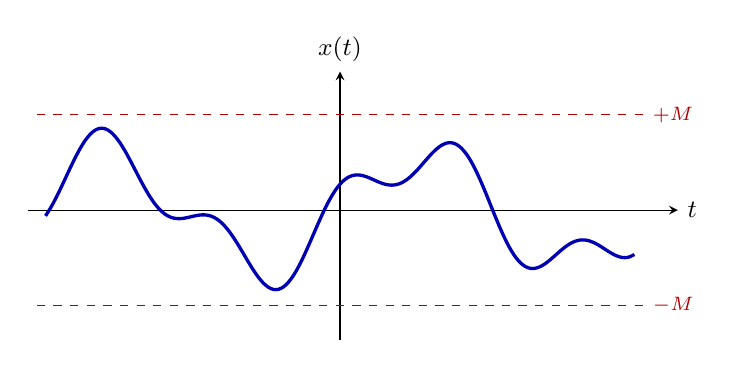
\begin{tikzpicture}[x=1.1cm,y=1.1cm,>=stealth]
  \draw[->] (-3.6,0) -- (3.9,0) node[right,font=\small] {$t$};
  \draw[->] (0,-1.5) -- (0,1.6) node[above,font=\small] {$x(t)$};
  \draw[dashed,red!70!black] (-3.5,1.1) -- (3.5,1.1) node[right,font=\scriptsize] {$+M$};
  \draw[dashed,red!70!black] (-3.5,-1.1) -- (3.5,-1.1) node[right,font=\scriptsize] {$-M$};
  \draw[very thick,blue!70!black,smooth,samples=120,domain=-3.4:3.4] plot (\x,{0.65*sin(\x*100)+0.3*cos(\x*260)});
\end{tikzpicture}
\caption{有界信号：不管 $t$ 取多大多小，波形始终待在两条红色虚线之间。}
\end{figure}

\subsection{证明}
\begin{remember}
\textbf{证}稳定：设 $|x(t)|<M$，推出 $|y(t)|$ 被某个固定的数夹住。这个数可以很大，只要固定就行。

\textbf{证}不稳定：举一个有界的输入，让输出变成无界。
\end{remember}

\subsection{例题：稳定}
\example{\texorpdfstring{$y(t)=e^{x(t)}$}{y(t)=exp(x(t))}}{稳定}{}
\textbf{系统}：$x(t)\to y(t)=e^{x(t)}$。

\textbf{证明}。设输入有界：$|x(t)|<M$。则
\[
|y(t)|=\bigl|e^{x(t)}\bigr|=e^{x(t)}\ \le\ e^{|x(t)|}\ \le\ e^{M},
\]
其中第一处不等号用到 $x(t)\le|x(t)|$ 及 $e^{u}$ 单调递增。$e^{M}$ 是与 $t$ 无关的固定上界，故 $y(t)$ 有界，系统稳定。\hfill$\blacksquare$

\example{\texorpdfstring{$y(t)=x(t)^3-2x(t)^2+x(t)+1$}{y(t)=x(t)的3次-2倍x(t)的平方+x(t)+1}}{稳定}{}
\textbf{系统}：$x(t)\to y(t)=x(t)^3-2x(t)^2+x(t)+1$。

\textbf{证明}。设 $|x(t)|<M$。由三角不等式 $|a+b+c+d|\le|a|+|b|+|c|+|d|$（并注意 $|-2x^2|=2|x|^2$），
\begin{align*}
|y(t)|&=\bigl|x^3-2x^2+x+1\bigr|\\
&\le |x|^3+2|x|^2+|x|+1\\
&\le M^3+2M^2+M+1.
\end{align*}
$M^3+2M^2+M+1$ 是固定上界，故 $y(t)$ 有界，系统稳定。\hfill$\blacksquare$

多项式型系统都可用同一办法：把每一项的 $|x|$ 换成 $M$，得到的数只要固定，系统就稳定——与表达式看起来多「大」无关。

\subsection{例题：不稳定}
\begin{center}
\begin{tabular}{@{}p{3.9cm}p{1.5cm}p{8.6cm}@{}}
\toprule
系统 & 结论 & 反例\\
\midrule
微分器\newline $y(t)=\dfrac{\mathrm{d}x(t)}{\mathrm{d}t}$ & 不稳定 & 取 $x(t)=u(t)$（阶跃，被 $1$ 夹住）。它在 $t=0$ 处一下子升 $1$，求导得冲激 $\delta(t)$，在 $t=0$ 变成\textbf{无穷大}，夹不住\\
积分器\newline $y(t)=\displaystyle\int_{-\infty}^{t}x(\tau)\,\mathrm{d}\tau$ & 不稳定 & 取 $x(t)\equiv1$（被 $M=1$ 夹住）。从 $-\infty$ 积到 $t$，$y(t)=+\infty$，夹不住\\
累加器\newline $y[n]=\displaystyle\sum_{k=-\infty}^{n}x[k]$ & 不稳定 & 同样道理\\
\bottomrule
\end{tabular}
\end{center}

\begin{figure}[H]
\centering
\begin{tikzpicture}[>=stealth]
  % 左：微分器
  \begin{scope}[shift={(0,0)}]
    \draw[->] (-0.3,0) -- (2.4,0) node[right,font=\scriptsize] {$t$};
    \draw[->] (0.6,-0.1) -- (0.6,1.3);
    \draw[very thick,blue!70!black] (-0.3,0) -- (0.6,0) -- (0.6,0.8) -- (2.3,0.8);
    \node[font=\scriptsize,blue!70!black] at (1.5,1.1) {$x=u(t)$：有界};
    \draw[->,gray] (2.9,0.5) -- (3.6,0.5) node[midway,above,font=\tiny,gray] {求导};
  \end{scope}
  \begin{scope}[shift={(4.0,0)}]
    \draw[->] (-0.3,0) -- (2.4,0) node[right,font=\scriptsize] {$t$};
    \draw[->] (0.6,-0.1) -- (0.6,1.9);
    \draw[->,very thick,red!75!black] (0.6,0) -- (0.6,1.8);
    \node[font=\scriptsize,red!75!black,anchor=west] at (0.75,1.55) {$\delta(t)$：$\to\infty$};
  \end{scope}
  % 右：积分器
  \begin{scope}[shift={(8.6,0)}]
    \draw[->] (-0.3,0) -- (2.4,0) node[right,font=\scriptsize] {$t$};
    \draw[->] (0.6,-0.1) -- (0.6,1.3);
    \draw[very thick,blue!70!black] (-0.3,0.8) -- (2.3,0.8);
    \node[font=\scriptsize,blue!70!black] at (1.5,1.1) {$x\equiv1$：有界};
    \draw[->,gray] (2.9,0.5) -- (3.6,0.5) node[midway,above,font=\tiny,gray] {积分};
  \end{scope}
  \begin{scope}[shift={(12.6,0)}]
    \draw[->] (-0.3,0) -- (2.2,0) node[right,font=\scriptsize] {$t$};
    \draw[->] (0.6,-0.1) -- (0.6,1.9);
    \draw[->,very thick,red!75!black] (-0.2,0.1) -- (2.1,1.8);
    \node[font=\scriptsize,red!75!black,anchor=west] at (0.1,1.75) {$\to\infty$};
  \end{scope}
\end{tikzpicture}
\caption{左：微分器把一个有界的阶跃变成无穷大的冲激。右：积分器把一个有界的常数 $1$ 越积越大，没有上限。}
\end{figure}

\point{思考题。}
连续的微分器不稳定，但\textbf{离散的微分器}（差分 $y[n]=x[n]-x[n-1]$）是\textbf{稳定}的，想一想为什么。

\begin{skippable}
\textbf{解答}：设 $|x[n]|<M$，则 $|y[n]|\le|x[n]|+|x[n-1]|<2M$，被 $2M$ 夹住，所以稳定。连续微分器不稳定，是因为连续信号可以在一瞬间跳变（跳变处导数无穷大）；离散信号每个点都是有限的数，相邻两点相减，差不会无穷大。
\end{skippable}

%==================================================================
\section{综合习题：教材第 33 页习题 1-16}
做教材第 33 页习题 1-16，把五个性质综合起来用：

\begin{center}
\renewcommand{\arraystretch}{1.35}
\begin{tabular}{@{}lccccc@{}}
\toprule
系统 & 线性 & 时不变 & 无记忆 & 因果 & 稳定\\
\midrule
$y(t)=e^{x(t)}$ & $\times$ & $\checkmark$ & $\checkmark$ & $\checkmark$ & $\checkmark$\\
$y[n]=x[n]\,x[n-1]$ & $\times$ & $\checkmark$ & $\times$ & $\checkmark$ & $\checkmark$\\
$y(t)=\dfrac{\mathrm{d}x(t)}{\mathrm{d}t}$ & $\checkmark$ & $\checkmark$ & $\times$ & $\checkmark$ & $\times$\\
\bottomrule
\end{tabular}
\end{center}
（$\checkmark$ 表示「是」，$\times$ 表示「否」；最后一格为 $\times$。）

\subsection{第一行~\texorpdfstring{$y(t)=e^{x(t)}$}{y(t)=exp(x(t))}}
\begin{itemize}[nosep]
\item 线性\textbf{否}：看上去「每项有 $x$、$x$ 一次」，但 $e^{x}=1+x+\tfrac{x^2}{2!}+\cdots$ 不是一次；
\item 时不变\textbf{是}：$t$ 只在 $x$ 括号里，括号里只是 $t$；
\item 无记忆\textbf{是}：$y(t)$ 只依赖 $x(t)$；
\item 因果\textbf{是}：无记忆系统一定因果；
\item 稳定\textbf{是}：前面例 1 证过。
\end{itemize}

\subsection{第二行~\texorpdfstring{$y[n]=x[n]\,x[n-1]$}{y[n]=x[n]x[n-1]}}
\begin{itemize}[nosep]
\item 线性\textbf{否}：「这里两个 $x$ 了」，$x$ 不是一次；
\item 时不变\textbf{是}：$n$ 只在 $x$ 括号里，括号里是 $n$ 和 $n-1$（只平移）。
\item 无记忆\textbf{否}：$y[n]$ 还跟 $x[n-1]$ 有关；
\item 因果\textbf{是}：$x$ 括号里是 $n$ 和 $n-1$，都不大于 $y$ 括号里的 $n$；
\item 稳定\textbf{是}：$|x[n]x[n-1]|\le M\cdot M$，被 $M^2$ 夹住。
\end{itemize}

\subsection{第三行 微分器~\texorpdfstring{$y(t)=\dfrac{\mathrm{d}x(t)}{\mathrm{d}t}$}{y(t)=dx(t)/dt}}
\begin{itemize}[nosep]
\item 线性\textbf{是}，时不变\textbf{是}：前面都证明过（时不变的证明见例~\ref{ex:diff}）。
\item 无记忆\textbf{否}：要算 $\dfrac{\mathrm{d}x}{\mathrm{d}t}$，必须知道 $t\pm\Delta t$ 那么\textbf{一小点}地方的值；
\item 稳定\textbf{否}：前面讲过，微分器不稳定；
\item 因果：争议最大的一格，见下。
\end{itemize}

\point{微分器是因果的吗？}
这一格有争议：\textbf{写因果或非因果都有依据，按导数的两种等价算法可判为因果}。理由是导数是一个极限，可以有两种算法：

\begin{center}
\renewcommand{\arraystretch}{1.3}
\begin{tabular}{@{}p{3.8cm}p{5.6cm}p{4.2cm}@{}}
\toprule
算法 & 式子 & 按因果的定义\\
\midrule
取 $t$ \textbf{右边}一点点 & $\displaystyle\lim_{\Delta t\to0^+}\dfrac{x(t+\Delta t)-x(t)}{\Delta t}$ & 用到了 $t+\Delta t>t$ 的值，\textbf{非因果}\\
取 $t$ \textbf{左边}一点点 & $\displaystyle\lim_{\Delta t\to0^+}\dfrac{x(t)-x(t-\Delta t)}{\Delta t}$ & 用到的 $t-\Delta t<t$，\textbf{因果}\\
\bottomrule
\end{tabular}
\end{center}
推理：把 $y(t)$ 写成 $\dfrac{\mathrm{d}x(t)}{\mathrm{d}t}$ 本身就有一个\textbf{假设}：左极限和右极限\textbf{相等}（导数存在）。既然如此，虽然右边那个算法是非因果的，也能用底下这个因果的算法算出来，所以按这个角度它是因果的。


\begin{skippable}
\textbf{直观理解}：导数是「变化有多快」。要知道 $t$ 这一刻变化多快，既可以「看一眼刚才到现在涨了多少」（只用过去，因果），也可以「偷看一眼马上要涨多少」（用了未来，非因果）。导数存在时两种看法算出的数相同，因此可判为因果。
\end{skippable}

\subsection{小测验}
\textbf{小测验}：五分钟做五道题，逐格判断。

练习方法：盖住 $\checkmark/\times$，对每个系统逐格判断，用各节的判据：线性看「每项有 $x$、一次」；时不变看「$t$ 只在括号里、只是 $t$」；无记忆看「两个括号里的数一样」；因果看「$x$ 括号里的数恒不大于 $y$ 括号里的」；稳定看「能不能用 $M$ 夹住」。

\end{document}
